\chapter{Funciones de Bessel}
\section{Ecuaci'on de Bessel}
Consideraremos aqu'i la ecuaci'on diferencial de Bessel con argumento complejo, $z\in\mathbb{C}$, ya que sus soluciones suminitrar'an funciones que satisfacen la E.D.O. de Bessel con variables reales y la E.D.O. modificada de Bessel. Finalmente, buscaremos soluciones de la ecuaci'on con un coeficiente $\nu^ 2$ real y positivo, pero no necesariamente entero.

En resumen, buscamos soluciones de la ecuaci'on
\begin{equation}\label{Besselec1}
z\frac{d\ }{dz}\left(z\frac{dy}{dz}\right)+(z^2-\nu^2)y(z)=0,
\end{equation}
que puede ser escrita como
\begin{equation}\label{EDOBessel}
y'' + \frac{1}{z} y' + \left( 1 - \frac{\nu^2}{z^2} \right)y = 0.
\end{equation}


\section{Soluci'on en serie en torno a $z = 0$}\label{secsolBess}
Buscaremos soluciones en serie de potencias de \eqref{Besselec1}. Es conveniente encontrar una serie en torno a $z=0$ (el ``punto m'as sim'etrico de la ecuaci'on''). Sin embargo, este punto es un punto singular de la ecuaci'on, por lo que en general no es posible expresar la soluci'on como una serie de la forma $y(z) = \sum_{n=0}^\infty a_n z^n$. Para entender esto m'as claramente, recuerde que los coeficientes $a_n$ ser'ian entonces proporcionales a la $n-$'esima derivada de la soluci'on $y(z)$, evaluada en $z=0$. Por lo tanto, encontrar la soluci'on de esta forma es equivalente a requerir que cada una de las derivadas de la soluci'on sean finitas en $z=0$. Como la E.D.O. es de segundo orden, se requieren dos condiciones iniciales, que pueden elegirse como $y(0)$ e $y'(0)$. Las derivadas superiores quedan determinadas por la E.D.O. Sin embargo, vemos de 
\eqref{EDOBessel} que $y''(0)$ (y las derivadas superiores) ser'a en general divergente, a'un en el caso en que se elija $y'(0)$, debido al t'ermino $({\nu^2}/{z^2})y(z)$. 

Afortunadamente, s'i es posible encontrar soluciones de la forma\footnote{Una forma alternativa de verificar que este es el caso es realizar el cambio de variable $y(z):=x^\alpha f(z)$ y ajustar la constante $\alpha$ de modo que la E.D.O. resultante para la funci'on $f(z)$ s'i pueda expresarse como una serie de potencias de la forma $f(z) = \sum_{n=0}^\infty b_n z^n$.}
\begin{equation}\label{yzasum}
y(z) = z^\alpha \sum_{n=0}^\infty a_n z^n = \sum_{n=0}^\infty a_n z^{n+\alpha},
\end{equation}
donde $\alpha$ es una constante (no necesariamente un entero) que ser'a elegida convenientemente. Asumiendo \eqref{yzasum}, las derivadas de $y(z)$ adoptan la forma siguiente:
\begin{equation}
y' = \sum_{n=0}^\infty (n+\alpha) a_n z^{n+\alpha-1}, \quad
y'' = \sum_{n=0}^\infty (n+\alpha)(n+\alpha-1) a_n z^{n+\alpha-2}.
\end{equation}

Substituyendo estas expansiones en \eqref{EDOBessel} encontramos
\begin{align}
0 &=  z^2 y'' + z y' + \left( z^2 - \nu^2 \right) y  \\
  &= \sum_{n=0}^\infty (n+\alpha)(n +\alpha - 1)\, a_n z^{n+\alpha}
  + \sum_{n=0}^\infty (n+\alpha)\, a_n z^{n+\alpha} + \sum_{n=0}^\infty a_n z^{n+\alpha+2}
  - \nu^2\sum_{n=0}^\infty a_n z^{n+\alpha}  \\
 &=  \sum_{n=0}^\infty \left[ (n+\alpha)^2 -\nu^2 \right] a_n z^{n+\alpha}
  + \sum_{n=2}^\infty a_{n-2} z^{n+\alpha} \\
 &= (\alpha^2-\nu^2)a_0\,z^\alpha+\left[ (\alpha+1)^2 -\nu^2 \right] a_1\,z^{\alpha+1}
 + \sum_{n=2}^\infty \left[ \left( (n+\alpha)^2 -\nu^2 \right) a_n+a_{n-2}\right]  z^{n+\alpha}.
\end{align}
Por lo tanto, los coeficientes deben satisfacer las siguientes condiciones:
\begin{equation}\label{rrBess}
(\alpha^2-\nu^2)a_0=0,  \qquad \left[ (\alpha+1)^2 -\nu^2 \right] a_1=0, \qquad 
\left( (n+\alpha)^2 -\nu^2 \right) a_n+a_{n-2}=0.
\end{equation}
Encontramos as'i una relaci'on de recurrencia entre $a_n$ y $a_{n-2}$, que permite entonces expresar todos los coeficientes $a_n$ con $n$ par en t'erminos de $a_0$ y todos los con $n$ impar en t'erminos de $a_1$. 

Como buscamos soluciones no nulas, asumimos primero que $a_0\neq 0$. Entonces la primera condici'on en \eqref{rrBess} implica que $\alpha=\pm\nu$. En este caso la segunda condici'on en \eqref{rrBess} se reduce a $(1+2\alpha)a_1=0$. Analizaremos primero el caso gen'erico en que $\alpha\neq -1/2$. Entonces necesariamente $a_1=0$ y s'olo los coefientes pares, de la forma $a_{2k}$, $k=0,1,2,\cdots$, ser'an no nulos. De la relaci'on de recurrencia en \eqref{rrBess} obtenemos
\begin{equation}\label{anan-2}
a_n=-\frac{a_{n-2}}{n(n+2\alpha)}.
\end{equation}
Aplicaci'on sucesiva de \eqref{anan-2} conduce a
\begin{align}
a_{2 k} &= \frac{a_0(-1)^k}{2^{2k}k!}\frac{1}{(1+\alpha)(2+\alpha)(3+\alpha)\cdots (k+\alpha)}\\
&= \frac{a_0 (-1)^k}{2^{2k} k!}\frac{\Gamma(1+\alpha)}{\Gamma(k +\alpha+ 1) }, \qquad k=0,1,2,\cdots. 
\end{align}
Aqu'i hemos introducido la funci'on Gamma. Por lo tanto, para $\alpha=\nu$ hemos encontrado una soluci'on de la forma
\begin{equation}
y_\nu(z) = a_0 \sum_{k=0}^\infty \frac{(-1)^k}{2^{2k}k!}\frac{\Gamma(1+\nu)}{\Gamma(k+\nu+ 1) }
z^{2k+\nu},
\end{equation}
donde $a_0$ es una constante arbitraria. Es conveniente definir las \textit{funciones de Bessel de primera especie y orden} $\nu$, $J_\nu(z)$, como las soluciones correspondientes al caso en que $a_0:=1/2^{\nu}\Gamma(\nu+1)$, de modo que
\begin{equation}\label{Besselnu}
\boxed{J_\nu(z) = \sum_{k = 0}^\infty \frac{ (-1)^k }{ k! \Gamma(k + \nu + 1) }
\left( \frac{z}{2} \right)^{2k+\nu}.}
\end{equation}

Expandiendo los primeros t'erminos, encontramos:
\begin{align}\label{J-nu}
J_\nu(z) &= \frac{1}{\Gamma(\nu+1)}\left(\frac{z}{2}\right)^{\nu}
-\frac{1}{\Gamma(\nu+2)}\left(\frac{z}{2}\right)^{\nu+2}+ \cdots \\
&= \frac{1}{\Gamma(\nu+1)}\left(\frac{z}{2}\right)^{\nu}\left[1-\frac{1}{(\nu+1)}\left(\frac{z}{2}\right)^2+\cdots \right].
\end{align}



Como la E.D.O. de Bessel \eqref{Besselec1} depende del cuadrado de $\nu$, tendremos que 
\begin{equation}
J_{-\nu}(z) = \sum_{k = 0}^\infty \frac{ (-1)^k }{ k! \Gamma(k-\nu+1) }
\left( \frac{z}{2} \right)^{2k-\nu},
\end{equation}
es tambi'en una soluci'on (que equivale al caso $\alpha=-\nu$). 

\textit{Si $\nu$ es positivo, pero no es entero}, entonces tanto $\Gamma(k+\nu+1)$ como $\Gamma(k-\nu+1)$ asumen valores finitos y por lo tanto $J_\nu$ y $J_{-\nu}$ est'an bien definidas para todo $z$. Para valores de $z$ cercanos a cero tendremos entonces que $J_\nu\approx (z/2)^\nu/\Gamma(1+\nu)$ y $J_{-\nu}\approx (z/2)^{-\nu}/\Gamma(1-\nu)$. Por lo tanto, $J_\nu(0)=0$ mientras que  $J_{-\nu}(0)$ es divergente. Por otro lado, $J_0(0)=1$. En particular, esto muestra que $J_\nu$ y $J_{-\nu}$ \textit{son linealmente independientes si $\nu$ no es entero}.
En este caso la soluci'on general de \eqref{Besselec1} es de la forma
\begin{equation}
y(z)=c_1J_\nu(z)+c_2J_{-\nu}(z).
\end{equation}
Por razones hist'oricas y de conveniencia futura se definen adicionalmente las \textbf{funciones de Bessel de segunda especie} de orden $\nu$, tambi'en llamadas \textbf{funciones de Neumann} de orden $\nu$, $N_\nu(z)$, por
\begin{equation}
N_\nu(z):=\frac{\cos(\pi\nu)J_\nu(z)-J_{-\nu}(z)}{\sen(\pi\nu)}.
\end{equation}
Entonces la soluci'on general de \eqref{Besselec1} puede expresarse como una combinaci'on lineal de la funci'on de Bessel y de Neumann correspondiente:
\begin{equation}
y(z)=c_3J_\nu(z)+c_4N_\nu(z).
\end{equation}

\subsubsection{Caso en que $\alpha^2\neq\nu^2$}
Asumiendo ahora que $\alpha^2\neq\nu^2$, entonces $a_0=0$ con lo cual $a_{2k}= 0$, con esto $a_1\neq 0$ luego $(\alpha+1)^2-\nu^2=0$. Reemplazando esto \'utlimo en \eqref{rrBess}, se tiene que
\begin{equation} \label{rrBEssimpar}
a_n=-\frac{a_{n-2}}{(n-1)(n+1+2\alpha)}.
\end{equation}
Aplicando sucesivamente \eqref{rrBEssimpar}, se tiene que
\begin{eqnarray}
a_{2k+1}&=&\frac{(-1)^ka_1}{2^{2k}k!}\frac{1}{(\alpha+2)(\alpha+3)(\alpha+4)\cdots (\alpha +k+1)}\\
&=&\frac{(-1)^ka_1}{2^{2k }k!}\frac{\Gamma(\alpha+2)}{\Gamma(\alpha+k+2)}
\end{eqnarray}

As\'i, para $\alpha=\nu-1$ se tiene que la soluci\'on toma la forma
\begin{equation}
y_\nu(z) = a_1 \sum_{k=0}^\infty \frac{(-1)^k}{2^{2k}k!}\frac{\Gamma(1+\nu)}{\Gamma(k+\nu+ 1) }
z^{2k+\nu}
\end{equation}

Eligiendo $a_1=1/(2^{\nu}\Gamma(1+\nu))$, se obtiene nuevamente la funci\'on de Bessel de primera especie, dada por \eqref{Besselnu}

\subsubsection{Caso en que $\alpha=-\frac{1}{2}$}

En este caso $a_0\neq 0$ y $a_1\neq 0$, de \eqref{rrBess} se tiene la siguiente relaci\'on de recurrencia
\begin{equation}
a_n=-\frac{a_{n-2}}{n(n-1)}.
\end{equation} 

Si $n$ es par entonces
\begin{equation}
a_{2k}=\frac{(-1)^k a_0}{(2k)!}.
\end{equation}

Si $n$ es impar entonces
\begin{equation}
a_{2k+1}=\frac{(-1)^k a_1}{(2k+1)!}.
\end{equation}

As\'i, en la soluci\'on se tiene los siguiente
\begin{eqnarray}
y(z)&=&z^{-1/2}\left(\sum_{k=0}^{+\infty}a_{2k}z^{2k}+\sum_{k=0}^{+\infty}a_{2k+1}z^{2k+1} \right)\\
&=&z^{-1/2}\left(a_0\sum_{k=0}^{+\infty}\frac{(-1)^k}{(2k)!}z^{2k}+a_1\sum_{k=0}^{+\infty}\frac{(-1)^k}{(2k+1)!}z^{2k+1} \right).
\end{eqnarray}

Por lo tanto, la soluci\'on de la E.D.O. de Bessel en este caso toma la siguiente forma
\begin{equation}
\boxed{y(z)= z^{-1/2}\left(a_0\cos(z)+a_1\sen(z) \right).}
\end{equation}



\subsubsection{Funci'on Gamma}
\begin{equation}
\Gamma(z):=\lim_{n\to\infty}\frac{1\cdot 2\cdot 3\cdots n}{z(z+1)(z+2)\cdots (z+n)}n^z,
\end{equation}
\begin{equation}
\Gamma(z):=\int_0^\infty e^{-t}t^{z-1}dt, \qquad \Re(z)>0,
\end{equation}
\begin{equation}
\frac{1}{\Gamma(z)}:=ze^{\gamma z}\prod_{n=1}^\infty \left(1+\frac{z}{n}\right)e^{-z/n},
\end{equation}
donde $\gamma=0.577216\cdots$ es la constante de Euler-Mascheroni\footnote{$\gamma:=\lim_{n\to\infty}\left(1+{1}/{2}+{1}/{3}+\cdots {1}/{n}-\ln n\right)$.}.
\begin{equation}
\Gamma(z+1)=z\Gamma(z),
\end{equation}
\begin{equation}
\Gamma(1+n)=n!, \qquad n=0,1,2,\cdots ,
\end{equation}
\begin{equation}\label{GzG1-z}
\Gamma(z)\Gamma(1-z)=\frac{\pi}{\sen(z\pi)}.
\end{equation}
\begin{equation}
\Gamma(-n)\to\pm\infty, \qquad n=0,1,2,\cdots .
\end{equation}
\begin{equation}
\Gamma(1/2)=\sqrt{\pi}.
\end{equation}
\begin{figure}[H]
\centering
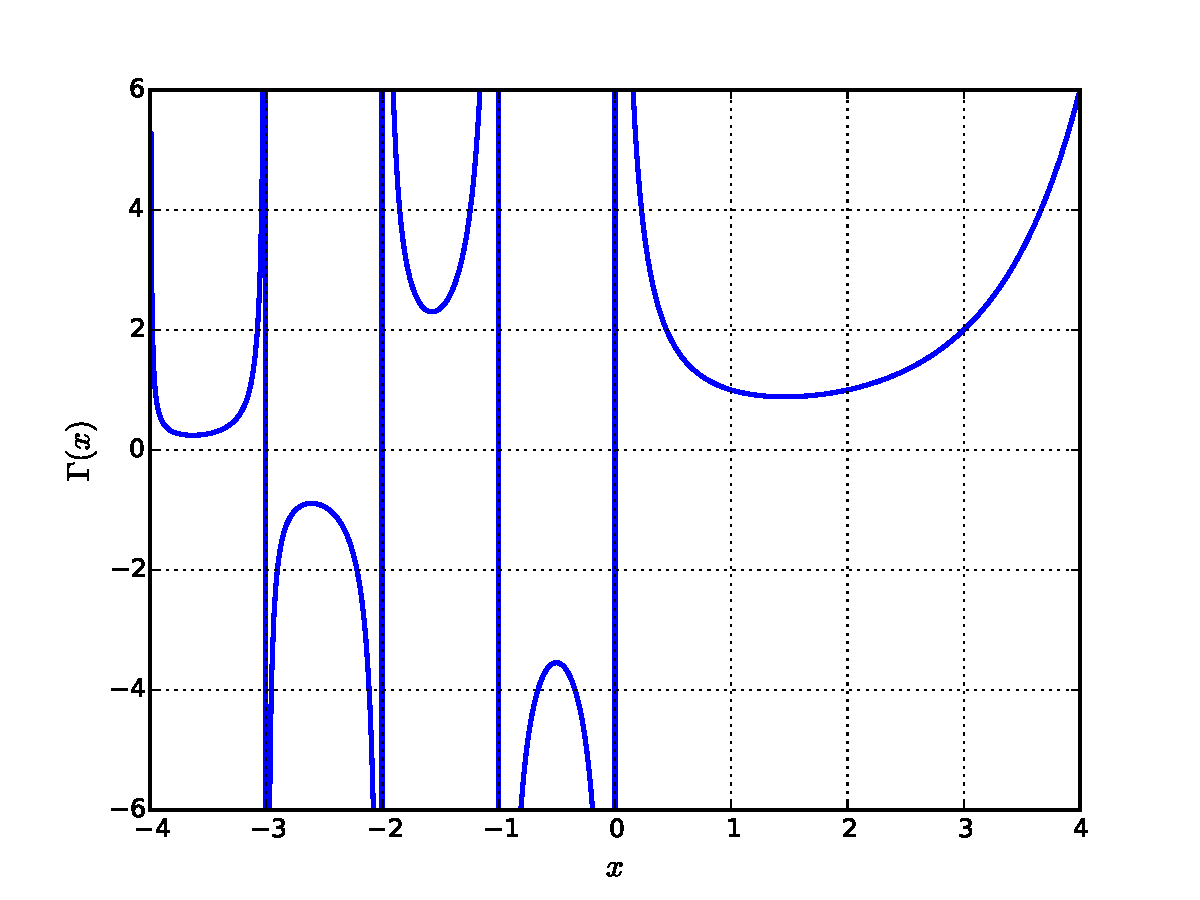
\includegraphics[angle=0,width=0.7\textwidth]{figs/fig-funcion-Gamma.pdf}
\caption{La funci'on $\Gamma$ con argumento real.}
\label{fig-Gamma}
\end{figure}


\section{Relaciones de Recurrencia}
Las funciones de Bessel $J_\nu(z)$ satisfacen las siguientes relaciones de recurrencia:
\begin{equation}\label{rrJnu1}
J_{\nu-1}(z)+J_{\nu+1}(z)=\frac{2\nu}{z}J_\nu(z),
\end{equation}
\begin{equation}\label{rrJnu2}
J_{\nu-1}(z)-J_{\nu+1}(z)=2J'_\nu(z).
\end{equation}
Podemos verificar estas relaciones usando directamente la expresi'on en serie de potencias \eqref{Besselnu}. En efecto,
\begin{align}
J_{\nu-1}(z)+J_{\nu+1}(z) &= 
\sum_{k=0}^\infty\frac{(-1)^k}{k!\Gamma(k+\nu)}\left(\frac{z}{2}\right)^{2k+\nu-1} 
+\sum_{k=0}^\infty\frac{(-1)^k}{k!\Gamma(k+\nu+2)}\left(\frac{z}{2}\right)^{2k+\nu+1} \label{idJ1}\\
&= \frac{2}{z}\left[\sum_{k=0}^\infty\frac{(-1)^k}{k!\Gamma(k+\nu)}\left(\frac{z}{2}\right)^{2k+\nu} 
+\sum_{k=0}^\infty\frac{(-1)^k}{k!\Gamma(k+\nu+2)}\left(\frac{z}{2}\right)^{2k+\nu+2}\right] \\
&= \frac{2}{z}\left[\sum_{k=0}^\infty\frac{(-1)^k(k+\nu)}{k!\Gamma(k+\nu+1)}\left(\frac{z}{2}\right)^{2k+\nu} \right. \nonumber\\
&\ \left.\qquad\qquad +\sum_{k=1}^\infty\frac{(-1)^{k-1}}{(k-1)!\Gamma(k+\nu+1)}\left(\frac{z}{2}\right)^{2k+\nu}\right] \\
&= \frac{2}{z}\left[\sum_{k=0}^\infty\frac{(-1)^k(k+\nu)}{k!\Gamma(k+\nu+1)}\left(\frac{z}{2}\right)^{2k+\nu}  +\sum_{k=1}^\infty\frac{(-1)^{k-1}}{\Gamma(k+\nu+1)}\frac{k}{k!}\left(\frac{z}{2}\right)^{2k+\nu}\right] \\
&= \frac{2}{z}\sum_{k=0}^\infty\frac{(-1)^k}{k!\Gamma(k+\nu+1)}\left[(k+\nu)-k\right]\left(\frac{z}{2}\right)^{2k+\nu} \label{idJ2}\\
&= \frac{2\nu}{x}\sum_{k=0}^\infty\frac{(-1)^k}{k!\Gamma(k+\nu+1)}\left(\frac{z}{2}\right)^{2k+\nu} \\
&= \frac{2\nu}{z}J_\nu(z).
\end{align}
De manera an'aloga, realizando ahora la resta de $J_{\nu-1}(z)$ y $J_{\nu+1}(z)$ obtenemos (ver \eqref{idJ1} y \eqref{idJ2}):
\begin{align}
J_{\nu-1}(z)-J_{\nu+1}(z) &= 
\sum_{k=0}^\infty\frac{(-1)^k}{k!\Gamma(k+\nu)}\left(\frac{z}{2}\right)^{2k+\nu-1} 
-\sum_{k=0}^\infty\frac{(-1)^k}{k!\Gamma(k+\nu+2)}\left(\frac{z}{2}\right)^{2k+\nu+1} \\
&= \frac{2}{z}\sum_{k=0}^\infty\frac{(-1)^k}{k!\Gamma(k+\nu+1)}\left[(k+\nu)+k\right]\left(\frac{z}{2}\right)^{2k+\nu}\\
&= \sum_{k=0}^\infty\frac{(-1)^k}{k\Gamma(k+\nu+1)}(2k+\nu)\left(\frac{z}{2}\right)^{2k+\nu-1}\\
&= \frac{d\ }{dz}\sum_{k=0}^\infty\frac{(-1)^k}{k!\Gamma(k+\nu+1)}\left(\frac{z}{2}\right)^{2k+\nu} \\
&= J'_\nu(z).
\end{align}
A partir de las relaciones \eqref{rrJnu1} y \eqref{rrJnu2} podemos derivar otras relaciones. Por ejemplo, sumando \eqref{rrJnu1} y \eqref{rrJnu2} llegamos a
\begin{align}
J_{\nu-1}(z) &= J'_{\nu}(z)+\frac{\nu}{z}J_\nu(z) \label{Jnu-1JpJ}\\
&= z^{-\nu}\frac{d\ }{dz}\left[z^\nu J_\nu(z)\right]. \label{Jnu-1JpJ2}
\end{align}
Similarmente, la suma de \eqref{rrJnu1} y \eqref{rrJnu2} conduce a 
\begin{align}
J_{\nu+1}(z) &= -J'_{\nu}(z)+\frac{\nu}{z}J_\nu(z) \label{rrJni+1} \\
&= -z^{\nu}\frac{d\ }{dz}\left[z^{-\nu} J_\nu(z)\right]. \label{rrJni+2}
\end{align}
Finalmente, podemos verificar que estas relaciones implican que las funciones $J_\nu(z)$ satisfacen la ecuaci'on de Bessel. A partir de \eqref{Jnu-1JpJ} tenemos que $zJ'_\nu=zJ_{\nu-1}-\nu J_\nu$. Derivando y multiplicando por $z$ esta relaci'on, tenemos que
\begin{align}
z\frac{d\ }{dz}(zJ'_\nu) &= z\left(J_{\nu-1}+zJ'_{\nu-1}-\nu J'_\nu\right)\\
&= zJ_{\nu-1}+z^2J'_{\nu-1}-\nu zJ'_\nu. \label{zdzJ'}
\end{align}
Usando \eqref{rrJni+1} (reemplazando $\nu$ por $\nu-1$) para reescribir el segundo t'ermino de \eqref{zdzJ'} y nuevamente \eqref{Jnu-1JpJ} en el 'ultimo t'ermino, llegamos a
\begin{align}
z\frac{d\ }{dz}(zJ'_\nu) &= zJ_{\nu-1}+z\left[(\nu-1)J_{\nu-1}-zJ_\nu\right]-\nu (zJ_{\nu-1}-\nu J_\nu) \\
&= -(x^2-\nu^2) J_\nu,
\end{align}
que es equivalente a la ecuaci'on \eqref{Besselec1}.

\subsection{Representaci'on integral}
Las funciones de Bessel de orden $\nu$ y argumento real pueden expresarse como la siguiente integral en el plano completo
\begin{equation}\label{RIJnu}
\boxed{J_\nu(x)=2\pi i\int_{\cal C}e^{(x/2)(t-t^{-1})}t^{-\nu-1}dt,}
\end{equation}
donde $t\in\mathbb{C}$ est'a integrado sobre el contorno $\cal C$ indicado en la figura XXX.

Podemos probar esta relaci'on a partir de la siguiente representaci'on de la funci'on Gamma (ver, por ejemplo, la expresi'on (11.21) \cite{Hassani}):
\begin{equation}\label{1sGint}
\frac{1}{\Gamma(z)}=\frac{1}{2\pi i}\int_{\cal C}e^t t^{-z}dt.
\end{equation}

Primero, reescribimos el integrando de \eqref{RIJnu} como
\begin{align}
e^{(x/2)(t-t^{-1})}t^{-\nu-1} &= e^{xt/2}e^{-x/2t}t^{-\nu-1} \\
&= e^{xt/2}\left[\sum_{k=0}^\infty\frac{1}{k!}\left(\frac{-x}{2t}\right)^k\right]t^{-\nu-1} \\
&= \sum_{k=0}^\infty\frac{(-1)^k}{k!}\left(\frac{x}{2}\right)^ke^{xt/2}t^{-k-\nu-1}. \label{exttsum}
\end{align}
Entonces, integrando esta relaci'on sobre $\cal C$, encontramos
\begin{align}
\int_{\cal C}e^{(x/2)(t-t^{-1})}t^{-\nu-1}dt &= \sum_{k=0}^\infty\frac{(-1)^k}{k!}\left(\frac{x}{2}\right)^k\int_{\cal C}e^{xt/2}t^{-k-\nu-1}dt .
\end{align}
Finalmente, realizando el cambio de variable $x':=xt/2$ y usando \eqref{1sGint} reescribimos al 'ultima integral como
\begin{align}
\int_{\cal C}e^{xt/2}t^{-k-\nu-1}dt &= \frac{2}{x}\int_{\cal C}e^{t'}\left(\frac{2t'}{x}\right)^{-k-\nu-1}dt' \\
&= \left(\frac{2}{x}\right)^{-k-\nu}\int_{\cal C}e^{t'}t'^{-k-\nu-1}dt' \\
&= \left(\frac{2}{x}\right)^{-k-\nu}\frac{2\pi i}{\Gamma(k+\nu+1)}. \label{intCG2}
\end{align}
Sustituyendo \eqref{intCG2} en \eqref{exttsum} llegamos directamente al resultado deseado, luego de indentificar la expansi'on en serie de potencias \eqref{Besselnu} de la funci'on $J_\nu(x)$.

A partir de \eqref{RIJnu} podemos encotrar la expresi'on alternativa:
\begin{equation}
\boxed{J_\nu(x)=\frac{1}{\pi}\int_0^\pi\cos(\nu\theta-x\sen\theta)d\theta-\frac{\sen(\nu\pi)}{\pi}\int_0^\infty e^{-\nu t-x\senh t}dt.}
\end{equation}

\subsection{Forma asint'otica}
A partir de la representaci'on integral \eqref{RIJnu} es posible encontrar una expresi'on asint'otica para las funciones de Bessel, v'alida para valores ``grandes'' de $x$:
\begin{equation}\label{asinJnu}
J_\nu(x)\approx \sqrt{\frac{2}{\pi x}}\cos\left(x-\frac{\nu\pi}{2}-\frac{\pi}{4}\right), 
\qquad x\gg\left|\nu^2-\frac{1}{4}\right|.
\end{equation}

\subsection{Ceros de las funciones de Bessel}
Frecuentemente, es necesario evaluar las raices, o ceros, de las funciones de Bessel. La funci'on de Bessel $J_\nu(x)$ tiene infinitas raices (ver, por ejemplo, figura \ref{fig-Jn}). Denotaremos $\alpha_{\nu,n}$ a la $n$-'esima raiz de la funci'on $J_\nu(x)$, es decir, tal que $J_\nu(\alpha_{\nu,n})=0$ y $\alpha_{\nu,n+1}<\alpha_{\nu,n}$, $n=1,2,\cdots$. Los valores de estas raices son calculadas num'ericamente a partir, por ejemplo, de la expresi'on en serie \eqref{Besselnu} para las funciones de Bessel. En la tabla \ref{tabla:alphanun} se muestran algunas de estos ceros\footnote{Un sitio donde puede calcular en l'inea los ceros es: \url{http://cose.math.bas.bg/webMathematica/webComputing/BesselZeros.jsp}.}:
\begin{table}
\begin{center}
\begin{tabular}{cccccc}
\hline $\alpha_{m,n}$ & $m=0$ & $m=1$ & $m=2$ & $m=3$ \\ \hline 
$n=1$ & $2.4048$ & $3.8317$ & $5.1356$ & $6.3802$  \\ 
$n=2$ & $5.5201$ & $7.0156$ & $8.4172$ & $9.7610$  \\ 
$n=3$ & $8.6537$ & $10.1735$ & $11.6198$ & $13.0152$  \\ 
$n=4$ & $11.7915$ & $13.3237$ & $14.7960$ & $16.2235$  \\ 
$n=5$ & $14.9309$ & $16.4706$ & $17.9598$ & $19.4094$ \\
\hline 
\end{tabular} 
\caption{Las primeras ra'ices $\alpha_{m,n}$ de $J_m(x)$, $m=0,1,2,3,4$.}
\label{tabla:alphanun}
\end{center}
\end{table}

Es tambi'en frecuente requerir calcular las \textit{raices de las derivadas de las funciones de Bessel}. 'Estas ser'an denotadas por $\beta_{\nu,n}$ y entonces satisfacen $J'_\nu(\beta_{\nu,n})=0$ y $\beta_{\nu,n+1}<\alpha_{\beta,n}$, $n=1,2,\cdots$. La tabla  \ref{tabla:betanun} resume algunos de estos valores:
\begin{table}
\begin{center}
\begin{tabular}{cccccc}
\hline $\beta_{m,n}$ & $m=0$ & $m=1$ & $m=2$ & $m=3$ \\ \hline 
$n=1$ & $3.8317$ & $1.8412$ & $3.0542$ & $4.2012$  \\ 
$n=2$ & $7.0156$ & $5.3314$ & $6.7061$ & $8.0152$  \\ 
$n=3$ & $10.1735$ & $8.5363$ & $9.9695$ & $11.3459$ \\ 
\hline 
\end{tabular} 
\caption{Las primeras ra'ices $\beta_{m,n}$ de $J'_m(x)$, $m=0,1,2,3,4$.}
\label{tabla:betanun}
\end{center}
\end{table}

\subsection{Relaciones de Ortogonalidad}
Para $\nu\ge 0$, $\quad n,m=1,2,\cdots$ y $a>0$, tenemos que
\begin{equation}\label{roJnualpha}
\int_0^a J_\nu\left(\frac{\alpha_{\nu,n}}{a}\rho\right)J_\nu\left(\frac{\alpha_{\nu,m}}{a}\rho\right)\rho \, d\rho=\delta_{n,m}\frac{a^2}{2}\left[J_{\nu+1}(\alpha_{\nu,n})\right]^2.
\end{equation}
Similarmente,
\begin{equation}\label{roJnubeta}
\int_0^a J_\nu\left(\frac{\beta_{\nu,n}}{a}\rho\right)J_\nu\left(\frac{\beta_{\nu,m}}{a}\rho\right)\rho \, d\rho=\delta_{n,m}\frac{a^2}{2}\left(1-\frac{\nu^2}{\beta_{\nu,n}^2}\right)\left[J_\nu(\beta_{\nu,n})\right]^2.
\end{equation}

\section{Funciones de Bessel de orden entero}
\begin{figure}[H]
\centering
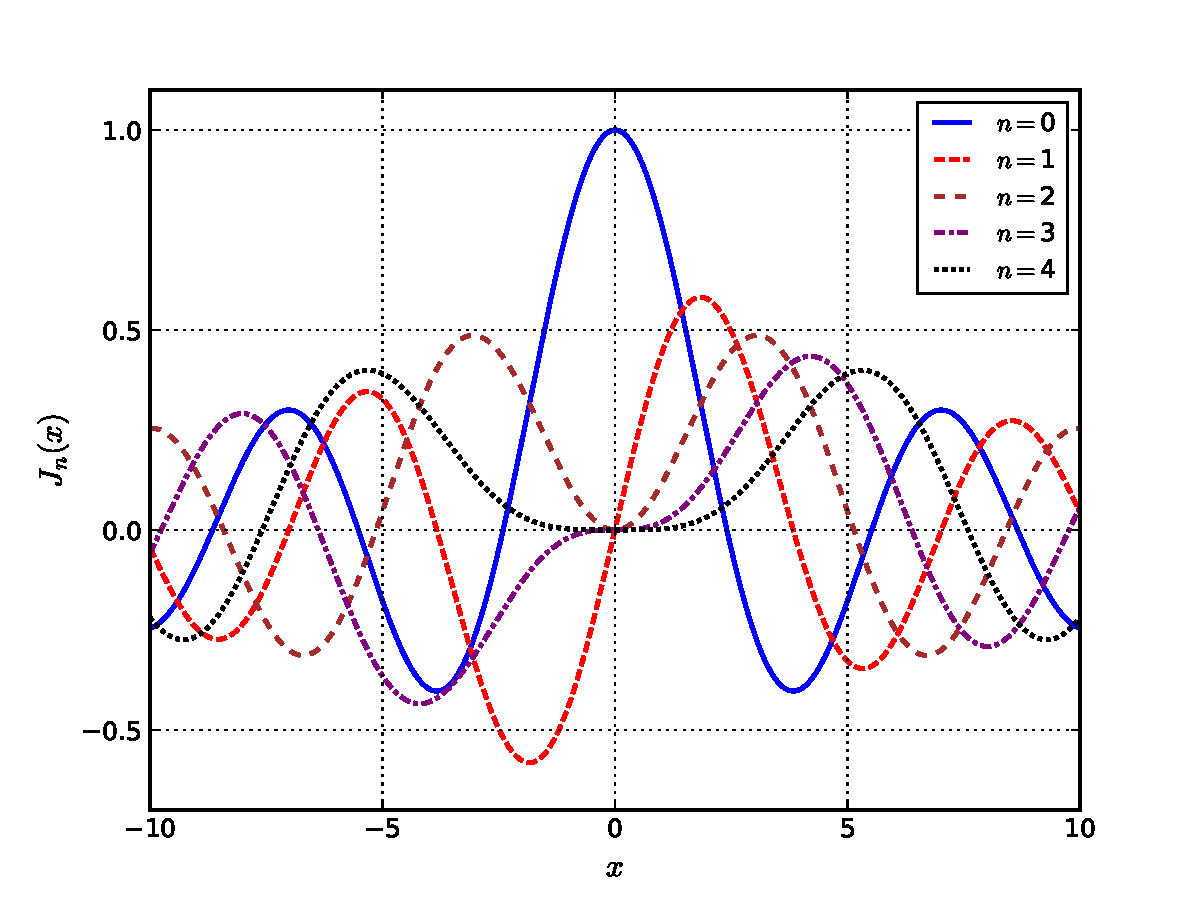
\includegraphics[angle=0,width=0.7\textwidth]{figs/fig-Bessel-J.pdf}
\caption{Primeras cinco funciones de Bessel de primera especie a orden entero.}
\label{fig-Jn}
\end{figure}
Consideremos las soluciones enteras de orden $n=0,1,2,\cdots$, entonces \eqref{Besselnu} se reduce a
\begin{align}
J_n(z) &= \sum_{k=0}^\infty \frac{(-1)^k}{k!\Gamma(k+n+ 1)}
\left(\frac{z}{2}\right)^{2k+n},
\end{align}
y como $\Gamma(k+n+ 1)$ tiene argumento entero, coincide con el factorial $(k+n)!$. Por lo tanto,
\begin{equation}
\boxed{J_n(z) =\sum_{k=0}^\infty \frac{(-1)^k}{k!(k+n)!}
\left(\frac{z}{2}\right)^{2k+n}.}
\end{equation}
Por otro lado, reemplazando $\nu=-n$, con $n=0,1,2,\cdots$, en \eqref{Besselnu} (o, equivalentemente $\nu=n$ en \eqref{J-nu}), obtenemos
\begin{align}\label{J-n}
J_{-n}(z) &= \sum_{k=0}^\infty \frac{(-1)^k}{k!\Gamma(k-n+ 1) }
\left(\frac{z}{2}\right)^{2k-n}.
\end{align}

Aqu'i hay que mirar cuidadosamente el caso en que $(k-n+ 1)$ asume valores enteros negativos, puesto que en esos casos la funci'on $\Gamma(k-n+ 1)$ diverge. Los casos en que $k-n+ 1=0,1,2,\cdots$ se presentan cuando $k=n-1,n-2,\cdots, 0$ respectivamente. Como $1/\Gamma(k-n+ 1)\to 0$ en estos casos\footnote{En otras palabras, estamos considerando (o definiendo) $J_{-n}$ como el l'imite de $J_{-\nu}$ cuando $\nu$ se acerca al entero $n$:  $J_{-n}(z):=\lim_{\nu\to n}J_{-\nu}(z)$.}, entonces los coeficientes de la suma en \eqref{J-n} tender'an a cero para todo $k=0,1,\cdots,n-1$. Por lo tanto, s'olo contribuir'an los t'erminos con $k\ge n$. Entonces \eqref{J-n} se reduce a
\begin{align}\label{J-n2}
J_{-n}(z) &= \sum_{k=n}^\infty \frac{(-1)^k}{k!\Gamma(k-n+ 1) }
\left(\frac{z}{2}\right)^{2k-n} \\
&= \sum_{k=0}^\infty \frac{(-1)^{k+n}}{(k+n)!\Gamma(k+1)}
\left(\frac{z}{2}\right)^{2k+n} \\
&= (-1)^n\sum_{k=0}^\infty \frac{(-1)^k}{(k+n)!k!}
\left(\frac{z}{2}\right)^{2k+n} \\
&= (-1)^n J_n(z).
\end{align}

Note adem'as que, como puede verse de su expresi'on en serie, las funciones $J_n(z)$ tienen paridad $n$, es decir,
\begin{equation}
J_n(-z)=(-1)^nJ_n(z).
\end{equation}

\subsection{Funci'on generadora de Funciones de Bessel de orden entero}
Consideramos la funci'on $g(t,z)$ definida por
\begin{equation}\label{defgtz}
g(t,z):=\sum_{n = -\infty}^\infty J_n(z) t^n, \qquad t,z\in \mathbb{C}.
\end{equation}
De esta forma, podemos entender a $g(t,z)$ como la \textit{funci'on generadora de las funciones de Bessel de orden entero}, por medio de la expansi'on (de Laurent) en potencias de $t$.

Para determinar la forma expl'icita de $g(t,z)$ podemos proceder como sigue. Derivamos \eqref{defgtz} con respecto a $z$ y usamos la relaci'on de recurrencia \eqref{rrJnu2} para expresar $J'_n(z)$ en t'erminos de  $J_{n-1}(z)$ y $J_{n+1}(z)$. Con esto, podemos escribir:
\begin{align}
\frac{\partial g}{\partial z} &= \sum_{n=-\infty}^\infty J'_n(z) t^n \\
&= \frac{1}{2}\sum_{n=-\infty}^\infty \left(J_{n-1}(z)-J_{n+1}(z)\right) t^n \\
&= \frac{1}{2}\left[t\sum_{n=-\infty}^\infty J_{n-1}(z)t^{n-1}-t^{-1}\sum_{n=-\infty}^\infty J_{n+1}(z)t^{n+1} \right]\\
&= \frac{1}{2}\left(t-t^{-1}\right)\sum_{n = -\infty}^\infty J_n(z) t^n\\
&= \frac{1}{2}\left(t-t^{-1}\right)g(t,z).
\end{align}
Podemos encontrar una expresi'on para la funci'on generadora a partir de esta relaci'on, consider'andola como una ecuaci'on diferencial para $g(t,z)$. La soluci'on es necesariamente de la forma
\begin{equation}\label{gtz2}
g(t,z)=f(t)\,e^{\frac{z}{2}\left(t-t^{-1}\right)}.
\end{equation}
Finalmente, la funci'on $f(t)$ puede determinarse evaluando \eqref{defgtz} para $z=0$ y luego comparando con \eqref{gtz2}:
\begin{equation}\label{gtz3}
g(t,0)=f(t)=\sum_{n = -\infty}^\infty J_n(0) t^n=J_0(0)=1.
\end{equation}
Aqu'i usamos el hecho que todas las funciones de Bessel de orden entero se anulan en $z=0$, excepto para $n=0$, ya que $J_0(0)=1$.
\begin{equation}\label{gtzJ}
\boxed{g(t,z)=e^{\frac{z}{2}\left(t-t^{-1}\right)}=\sum_{n = -\infty}^\infty J_n(z) t^n.}
\end{equation}

\subsection{Representaci'on integral}
Substituyendo $t=e^{i\theta}$ en \eqref{gtzJ} encontramos,
\begin{equation}\label{gteth}
\boxed{g(t,e^{i\theta})=e^{iz\sen\theta}=\sum_{n = -\infty}^\infty J_n(z) e^{in\theta}.}
\end{equation}
Esto significa que las \textit{funciones de Bessel son los coeficientes de la expansi'on en serie de Fourier de la funci'on} $e^{iz\sen\theta}$. Por lo tanto,
\begin{equation}
\boxed{J_n(z)=\frac{1}{2\pi}\int_0^{2\pi}e^{iz\sen\theta}e^{-in\theta}\,d\theta.}
\end{equation}
Equivalentemente, ya que el integrando es peri'odico de periodo $2\pi$, podemos desplazar el intervalo de integraci'on a $[-\pi,\pi]$, y escribir
\begin{equation}
J_n(z)=\frac{1}{2\pi}\int_{-\pi}^{\pi}e^{i(z\sen\theta-n\theta)}\,d\theta.
\end{equation}
Como $e^{i(z\sen\theta-n\theta)}=\cos(z\sen\theta-n\theta)+i\sen(z\sen\theta-n\theta)$, vemos que el integrando se divide en una contribuci'on par y otra impar en $\theta$. Por lo tanto,
\begin{equation}
\boxed{J_n(z)=\frac{1}{\pi}\int_0^{\pi}\cos(z\sen\theta-n\theta)\,d\theta.}
\end{equation}
En particular,
\begin{equation}
\boxed{J_0(z)=\frac{1}{2\pi}\int_{-\pi}^{\pi}e^{iz\sen\theta}\,d\theta=\frac{1}{\pi}\int_0^{\pi}\cos(z\sen\theta)\,d\theta.}
\end{equation}

\subsection{Sumatorias de funciones de Bessel}

Adicionalmente, de la relaci'on \eqref{gteth} podemos escribir,
\begin{align}
e^{iz\sen\theta} &= J_0(z)+\sum_{n=1}^\infty\left(J_n(z) e^{in\theta}+J_{-n}(z) e^{-in\theta}\right) \\
&=  J_0(z)+\sum_{n=1}^\infty\left(J_n(z) e^{in\theta}+(-1)^nJ_{n}(z) e^{-in\theta}\right) \\
&=  J_0(z)+\sum_{\substack{n=1 \\ n \text{ impar}}}^\infty J_n(z)\left(e^{in\theta}-e^{-in\theta}\right)+\sum_{\substack{n=2 \\ n \text{ par}}}^\infty J_n(z)\left(e^{in\theta}+e^{-in\theta}\right) \\
&=  J_0(z)+2i\sum_{\substack{n=1 \\ n \text{ impar}}}^\infty J_n(z)\sen(n\theta) +2\sum_{\substack{n=2 \\ n \text{ par}}}^\infty J_n(z)\cos(n\theta) \\
&=  J_0(z)+2i\sum_{n=1}^\infty J_{2n-1}(z)\sen[(2n-1)\theta] +2\sum_{n=1}^\infty J_{2n}(z)\cos(2n\theta).
\end{align}
Si el argumento de las funciones es real ($z=x$) entonces, igualando la parte real e imaginaria de ambos lados de la igualdad, obtenemos
\begin{equation}
\boxed{\cos(x\sen\theta)=J_0(x)+2\sum_{n=1}^\infty J_{2n}(x)\cos(2n\theta),}
\end{equation}
\begin{equation}
\boxed{\sen(x\sen\theta)=2\sum_{n=1}^\infty J_{2n-1}(x)\sen[(2n-1)\theta].}
\end{equation}

En particular, si $\theta=0$, obtenemos la relaci'on
\begin{equation}
J_0(x)+2\sum_{n=1}^\infty J_{2n}(x)=1.
\end{equation}

\section{Funciones de Bessel de orden semi-entero}
\begin{align}
J_{1/2}(z) &= \sum_{k=0}^\infty\frac{(-1)^k}{k!\Gamma(k+1/2+1)}
\left(\frac{z}{2}\right)^{2k+1/2} \\
&= \sum_{k=0}^\infty\frac{(-1)^k}{k!\Gamma(k+3/2)}
\left(\frac{z}{2}\right)^{2k+1/2} \\
&= \left(\frac{2}{\pi z}\right)^{1/2} \sum_{k=0}^\infty \frac{(-1)^k}
{(2k+1)!} z^{2k+1} \\
&= \left(\frac{2}{\pi z}\right)^{1/2} \sen z. \label{J1/2}
\end{align}
Aqu'i hemos usado
\begin{align}
\Gamma(k+\frac{3}{2}) &= (k+\frac{1}{2})\Gamma(k+\frac{1}{2}) \\
&= (k+\frac{1}{2})(k-\frac{1}{2})\Gamma(k-\frac{1}{2}) \\
&=  (k+\frac{1}{2})(k-\frac{1}{2})(k-\frac{3}{2})\Gamma(k-\frac{3}{2}) \\
&= \quad \cdots \\
&=  (k+\frac{1}{2})(k-\frac{1}{2})(k-\frac{3}{2})\frac{1}{2}\Gamma(\frac{1}{2}) \\
&= \frac{\sqrt{\pi}}{2^{k+1}} \underbrace{1\cdot 3\cdot 5\cdots (2k-1)(2k+1)}_{k+1\text{ t'erminos}} \\
&= \frac{\sqrt{\pi}}{2^{2k+1}}\frac{(2k+1)!}{k!}.
\end{align}

An'alogamente,
\begin{align}
J_{-1/2}(z) &= \sum_{k=0}^\infty\frac{(-1)^k}{k!\Gamma(k-1/2+1)}
\left(\frac{z}{2}\right)^{2k+1/2} \\
&= \sum_{k=0}^\infty\frac{(-1)^k}{k!\Gamma(k+1/2)}
\left(\frac{z}{2}\right)^{2k+1/2} \\
&= \left(\frac{2}{\pi z}\right)^{1/2} \sum_{k=0}^\infty \frac{(-1)^k}
{(2k)!} z^{2k} \\
&= \left(\frac{2}{\pi z}\right)^{1/2} \cos z, \label{J-1/2}
\end{align}
ya que
\begin{align}
\Gamma(k+\frac{1}{2}) &= \frac{\Gamma(k+\frac{3}{2})}{(k+\frac{1}{2}}) \\
&= \frac{\sqrt{\pi}}{2^{2k+1}}\frac{(2k+1)!}{(k+\frac{1}{2})k!}\\
&= \frac{\sqrt{\pi}}{2^{2k}}\frac{(2k)!}{k!}.
\end{align}

Podemos encontrar las otras funciones de Bessel de orden semi-entero usando las relaciones de recurrencia \eqref{rrJnu1} y \eqref{rrJnu2}. Por ejemplo
\begin{align}
    J_{3/2}(z)
    &= \frac{(1/2)}{z} J_{1/2}(z) - J_{1/2}'(z) 
    \\
    &= \frac{1}{2z} \left( \frac{2}{\pi} \right)^{1/2} z^{-1/2} \sen z
    - \left(-\frac{1}{2}\right) \left(\frac{2}{\pi}\right)^{1/2}
    z^{-3/2} \sen z - \left(\frac{2}{\pi}\right)^{1/2} z^{-1/2}
    \cos z 
    \\
    &= 2^{-1/2} \pi^{-1/2} z^{-3/2} \sen z
    + 2^{-1/2} \pi^{-1/2} z^{-3/2} \sen z
    - 2^{-1/2} \pi^{-1/2} \cos z 
    \\
    &= \left(\frac{2}{\pi}\right)^{1/2} z^{-3/2} \sen z
    - \left(\frac{2}{\pi}\right)^{1/2} z^{-1/2} \cos z 
    \\
    &= \left(\frac{2}{\pi}\right)^{1/2} \left( z^{-3/2} \sen z
      - z^{-1/2} \cos z \right).
  \end{align}



\section{Funciones de Bessel de segunda especie}\label{sec:FB2E}
Como hemos ya discutido en la secci'on \ref{secsolBess}, cuando $\nu$ no es un entero, las funciones de Bessel de segunda especie, tambi'en llamadas funciones de Neumann $N_\nu(z)$ ('o $Y_\nu(z)$), definidas por
\begin{equation}\label{defNnu}
N_\nu (z):=  \frac{J_\nu(z) \cos(\nu \pi) - J_{-\nu}(z)}{\sen(\nu \pi)} , \qquad \nu\neq n=0, \pm 1, \pm, 2, \cdots,
\end{equation}
son soluciones linealmente independientes de $J_\nu(z)$ de ecuaci'on de Bessel. Esta combinaci'on lineal particular es 'util puesto que, entre otras cosas, suministra una expresi'on complementaria a las funciones $J_\nu(z)$ en lo que respecta a su forma asint'otica. En efecto, a partir de \eqref{asinJnu} encontramos que
\begin{equation}\label{asinNnu}
\boxed{N_\nu(x)\approx \sqrt{\frac{2}{\pi x}}\sen\left(x-\frac{\nu\pi}{2}-\frac{\pi}{4}\right), 
\qquad x\gg\left|\nu^2-\frac{1}{4}\right|.}
\end{equation}
Adem'as, puede usarse la misma expresi'on \eqref{defNnu} en el caso en que $\nu$ es entero ($\nu=n$). Sabemos que en este caso, $J_{-n}(z)$ no es linealmente independiente de $J_{-n}(z)$ ya que se cumple que $J_{-n}(z)=(-1)^nJ_n(z)$. No obstante, podemos usar \eqref{defNnu} para encontrar la segunda soluci'on linealmente independiente $N_n(z)$, \textit{como el l'imite de \eqref{defNnu} cuando el par'ametro $\nu$ se acerca al entero $n$}, es decir,
\begin{equation}\label{Nnlim}
N_n(z):=  \lim_{\nu\to n}\frac{J_\nu(z) \cos(\nu \pi) - J_{-\nu}(z)}{\sen(\nu \pi)} , \qquad n=0, \pm 1, \pm, 2, \cdots .
\end{equation}
Note que los coeficientes de la combinaci'on lineal \eqref{defNnu} son tales que el l'imite es no trivial, ya que tanto el numerador como el denominador tienden a cero cuando $\nu$ tiende a $n$. Por esto, usando la regla de L'H\^opital, encontramos que
\begin{equation}\label{Nnder}
N_n(z)=\frac{1}{\pi}\left[\frac{\partial J_\nu(z)}{\partial\nu}-(-1)^n\frac{\partial J_{-\nu}(z)}{\partial\nu}\right]_{\nu=n}.
\end{equation}
Puede (h'agalo!) verificarse que la funci'on definida por \eqref{Nnder}, efectivamente satisface la ecuaci'on de Bessel \eqref{Besselec1}. Adem'as, de \eqref{Nnder} se sigue, usando $(\partial J_\nu/\partial\nu)_{\nu=-n}=-(\partial J_{-\nu}/\partial\nu)_{\nu=n}$, que
\begin{equation}
\boxed{N_{-n}(z)=(-1)^nN_n(z).}
\end{equation}
Por otro lado, de la expansi'on \eqref{J-nu} obtenemos que cerca de $z=0$, y para $\nu>0$,
\begin{equation}
N_\nu(z)\approx -\frac{1}{\sen(\nu\pi)}\frac{1}{\Gamma(1-\nu)}\left(\frac{2}{z}\right)^\nu=-\frac{1}{\pi}\Gamma{(\nu)}\left(\frac{2}{z}\right)^\nu.
\end{equation}
Aqu'i hemos usamos la identidad \eqref{GzG1-z}. Por lo tanto, para $\nu\to n$, obtenemos
\begin{equation}
N_n(z)\approx -\frac{1}{\pi}(n-1)!\left(\frac{2}{z}\right)^n, \qquad z\approx 0, \qquad n>0,
\end{equation}
de donde vemos que estas funciones divergen en el origen origen. Note que incluso $N_0(z)$ diverge en $z=0$, ya que\footnote{A partir de \eqref{Nnder}, se encuentra, usando la \textit{funci'on  digamma} $\Psi_0(z):=\Gamma'(z)/\Gamma(z)$, que: \begin{equation}
N_0(z)=\frac{2}{\pi}\left(\frac{\partial J_\nu}{\partial\nu}\right)_{\nu=0}=\frac{2}{\pi}\left[-\frac{\Psi_0(\nu+1)}{\Gamma(\nu+1)}\left(\frac{z}{2}\right)^\nu+\frac{1}{\Gamma(\nu+1)}\left(\frac{z}{2}\right)^\nu\ln\left(\frac{z}{2}\right)+\cdots\right]_{\nu=0}=\frac{2}{\pi}\left[-\Psi_0(1)+\ln\left(\frac{z}{2}\right)+\cdots\right].
\end{equation}}  
\begin{equation}
N_0(z)\approx \frac{2}{\pi}\left[\ln\left(\frac{z}{2}\right) + \gamma \right], \qquad z\approx 0,	
\end{equation}
donde $\gamma=-\Psi_0(1)$ es la constante de Euler-Mascheroni, $\gamma=0.5772\cdots$.


\subsection{Representaci'on integral}
\begin{equation}
N_n(x) =\frac{1}{\pi} \int_0^\pi \sen(x \sen\theta - n\theta) \, d\theta
- \frac{1}{\pi} \int_0^\infty\left[ e^{n t} + (-1)^n e^{-n t} \right]
 e^{-x \senh t} \, dt.
\end{equation}


\subsection{Relaciones de Recurrencia}
A partir de la definici'on \eqref{Nnlim} y las relaciones de recurrencia para las funciones de Bessel \eqref{rrJnu1} y \eqref{rrJnu2}, puede verificarse que las funciones de Bessel de segunda especie satisfacen \textit{las mismas relaciones de recurrencia que las de primera especie}:
\begin{equation}\label{rrNnu1}
N_{\nu-1}(z)+N_{\nu+1}(z)=\frac{2\nu}{z}N_\nu(z),
\end{equation}
\begin{equation}\label{rrNnu2}
N_{\nu-1}(z)-N_{\nu+1}(z)=2N'_\nu(z).
\end{equation}



\begin{figure}[H]
\centering
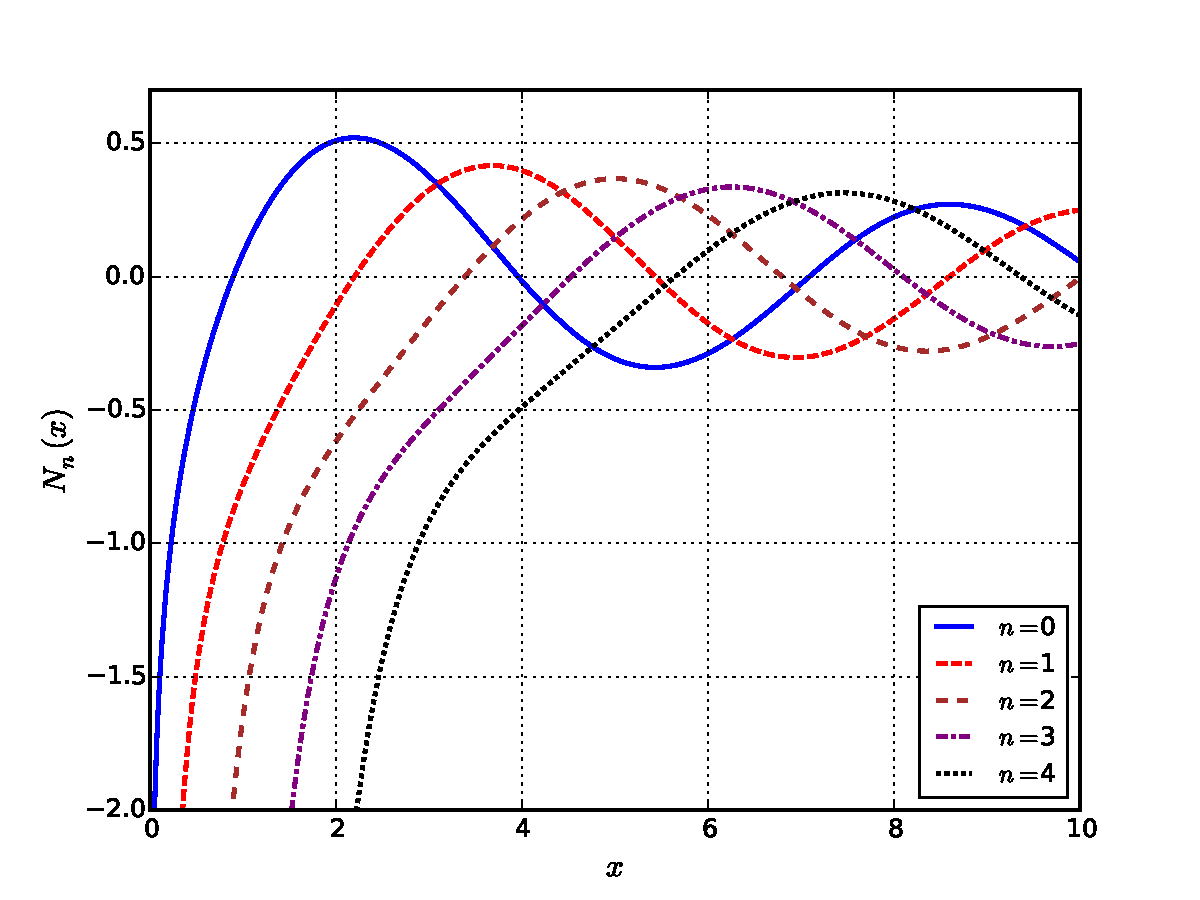
\includegraphics[angle=0,width=0.7\textwidth]{figs/fig-Bessel-N.pdf}
\caption{Primeras cinco funciones de Bessel de segunda especie (funciones de Neumann) de orden entero.}
\label{fig-Nn}
\end{figure}

\section{Funciones de Hankel}
En muchas aplicaciones f'isicas (especialmente cuando se estudian soluciones de la ecuaci'on de onda) es conveniente introducir otro par de funciones linealmente independientes, llamadas funciones de Hankel y denotadas por $H_\nu^{(1)}$ y $H_\nu^{(2)}$, definidas por
\begin{align}
  H_\nu^{(1)}(z) &:= J_\nu(z) + i N_\nu(z),  \\
  H_\nu^{(2)}(z) &:= J_\nu(z) - i N_\nu(z) .
\end{align}
%Wronskiano:
%\begin{equation} 
%W[H_\nu^{(1)}, H_\nu^{(2)}] = - \frac{i 4}{\pi z}. 
%\end{equation}
Las funciones de Hankel son linealmente independientes para todo $\nu$, y satisfacen las mismas relaciones de recurrencia que las funciones de Bessel.
La utilidad de su definici'on resulta clara al considerar su forma asint'otica. Usando \eqref{asinJnu} y \eqref{asinNnu} se encuentra que
\begin{equation}
H_\nu^{(1)}(x)\approx \sqrt{\frac{2}{\pi x}}\,e^{i(x-\nu\pi/2-\pi/4)}, \quad 
H_\nu^{(2)}(x)\approx \sqrt{\frac{2}{\pi x}}\,e^{-i(x-\nu\pi/2-\pi/4)}, 
\quad x\gg\left|\nu^2-\frac{\pi}{4}\right|.
\end{equation}

%\begin{align}
%H_\nu^{(1)}(x) &= \frac{e^{-\frac{1}{2} \nu\pi i}}{\pi i}\int_{-\infty}^{+\infty} e^{ix\cosh t - \nu t} \, dt, \\
%H_\nu^{(2)}(x) &= -\frac{e^{-\frac{1}{2} \nu\pi i}}{\pi i}\int_{-\infty}^{+\infty} e^{-ix\cosh t - \nu t} \, dt.
%\end{align}

\section{Funciones modificadas de Bessel}
La \textit{ecuaci'on modificada de Bessel} es 
\begin{equation} 
y'' + \frac{1}{x}y' -\left(1+\frac{\nu^2}{x^2}\right)y(x) = 0. 
\end{equation}
Las soluciones finitas en $x=0$ de esta ecuaci'on son de la forma $y(x)=J_\nu(ix)$. Como estamos especialmente interesados en el caso en que tanto $x$ como $y$ son reales, es conveniente  definir las \textit{funciones modificadas de Bessel de primera especia y orden} $\nu$:
\begin{equation}\label{defInu}
I_\nu(x) = i^{-\nu} J_\nu(ix). 
\end{equation}
La funci'on $I_\nu(x)$ as'i definida es real. En efecto, de la expansi'on en serie \eqref{Besselnu}
\begin{align}
  I_\nu(x) &= i^{-\nu} J_\nu(ix)   \\
  &= i^{-\nu}\sum_{k=0}^\infty\frac{(-1)^k}{k!\Gamma(k+\nu+1)}
  \left(\frac{ix}{2}\right)^{2k+\nu} \\
  &= i^{-\nu} \sum_{k=0}^\infty \frac{(-1)^k i^\nu i^{2k}}{k!\Gamma(k+\nu+1)} 
  \left(\frac{x}{2}\right)^{2+\nu}.
\end{align}
Por lo tanto,
\begin{equation}
\boxed{I_\nu(x) = \sum_{k=0}^\infty\frac{1}{k!\Gamma(k+\nu+ 1)}
  \left(\frac{x}{2}\right)^{2k+\nu}.}
\end{equation}
Nuevamente, $I_\nu$ y $I_{-\nu}$ son linealmente independientes, excepto si $\nu$ es entero, ya que en este 'ultimo caso se satisface que
\begin{equation}
I_{-n}(x)=I_n(z)
\end{equation}
\begin{figure}[H]
\centering
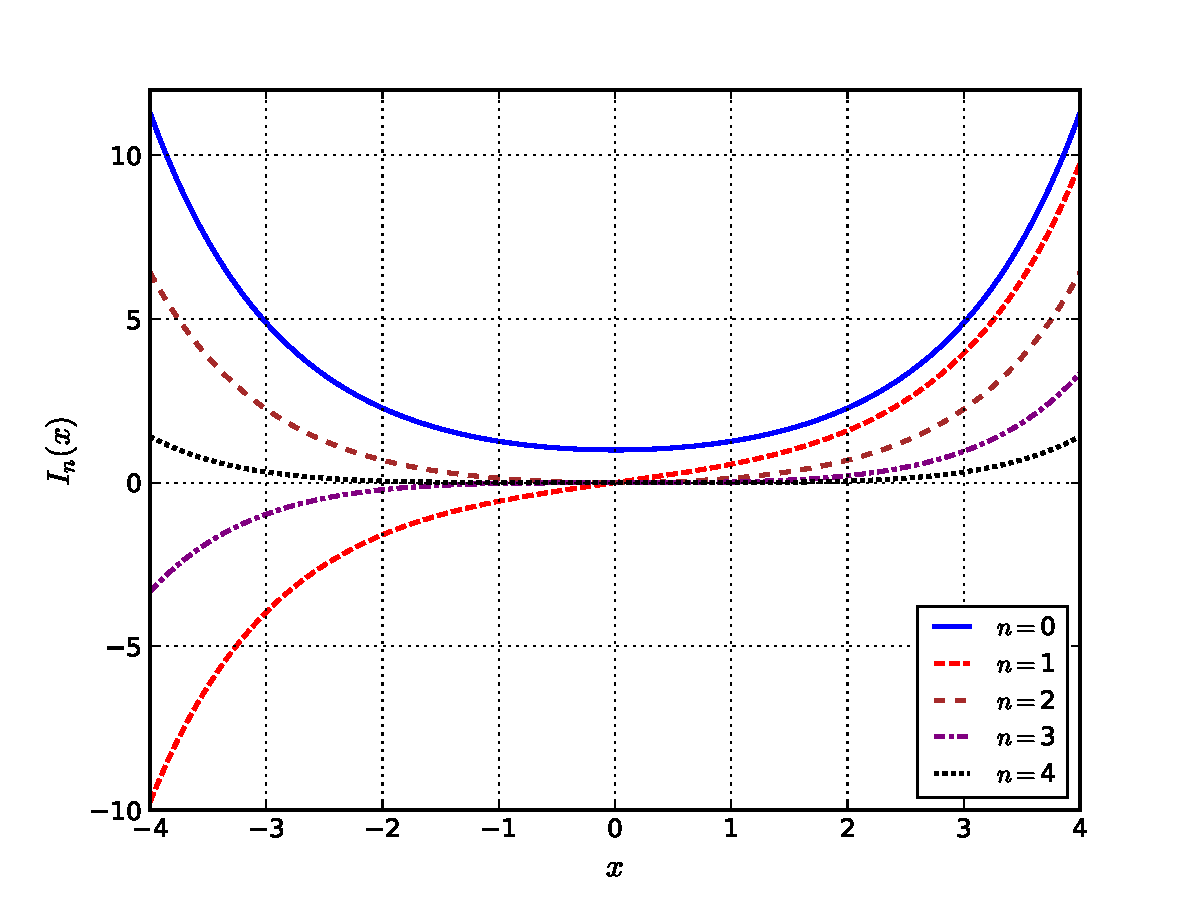
\includegraphics[angle=0,width=0.7\textwidth]{figs/fig-Bessel-I.pdf}
\caption{Primeras cinco funciones modificadas de Bessel (de primera especie) de orden entero.}
\label{fig-In}
\end{figure}
La correspondiente forma asint'otica de las funciones modificadas de Bessel $I_\nu(x)$ es
\begin{equation}
I_\nu(x) \approx \frac{1}{\sqrt{2\pi x}}\,e^x, \qquad x\gg\left|\nu^2-\frac{1}{4}\right|.
\end{equation}

Las funciones $I_\nu(x)$ satisfacen las siguientes relaciones de recurrencia, que se siguen a partir de \eqref{rrJnu1}, \eqref{rrJnu2} y \eqref{defInu}:
\begin{equation}\label{rrInu1}
I_{\nu-1}(x)+I_{\nu+1}(x)=2I'_\nu(x),
\end{equation}
\begin{equation}\label{rrInu2}
I_{\nu-1}(x)-I_{\nu+1}(x)=\frac{2\nu}{x}I_\nu(x).
\end{equation}

\subsection{Funciones Modificadas de Bessel de segunda especie}
En analog'ia con lo visto en la secci'on \ref{sec:FB2E}, es conveniente introducir las funciones de segunda especie, ahora denotadas por $K_\nu(x)$, y definidas de la forma siguiente:
\begin{equation}\label{defKnu}
K_\nu(x) := \frac{\pi}{2}\left[\frac{I_{-\nu}(x)-I_\nu(x)}{\sen(\nu\pi)}\right], \qquad \nu\neq n=0,\pm 1,\pm 2, \cdots.
\end{equation}
Note que como consecuencia de esta definici'on $K_{-\nu}(x)=K_\nu(x)$, por lo que es suficiente considerar $\nu\ge 0$.
Con estas definiciones, $I_\nu$ y $K_\nu$ son l.i. para todo $\nu$, y su forma asint'otica es nuevamente ``complementaria'' ya que
\begin{equation}
K_\nu(x) \approx \sqrt{\frac{\pi}{2x}} e^{-x}.
\end{equation}

En el caso de $\nu$ entero, la definici'on se realiza como el l'imite $\nu\to n$, es decir,
\begin{equation}
K_n(x) := \lim_{\nu\to n}\frac{\pi}{2}\left[\frac{I_{-\nu}(x)-I_\nu(x)}{\sen(\nu\pi)}\right], \qquad  n=0,1,2, \cdots.
\end{equation}
Usando nuevamente la regla de L'H\^opital, podemos escribir
\begin{equation}\label{Knder}
K_n(x)=\frac{(-1)^n}{2}\left[\frac{\partial I_{-\nu}(x)}{\partial\nu}-\frac{\partial I_\nu(x)}{\partial\nu}\right]_{\nu=n}.
\end{equation}

\begin{figure}[H]
\centering
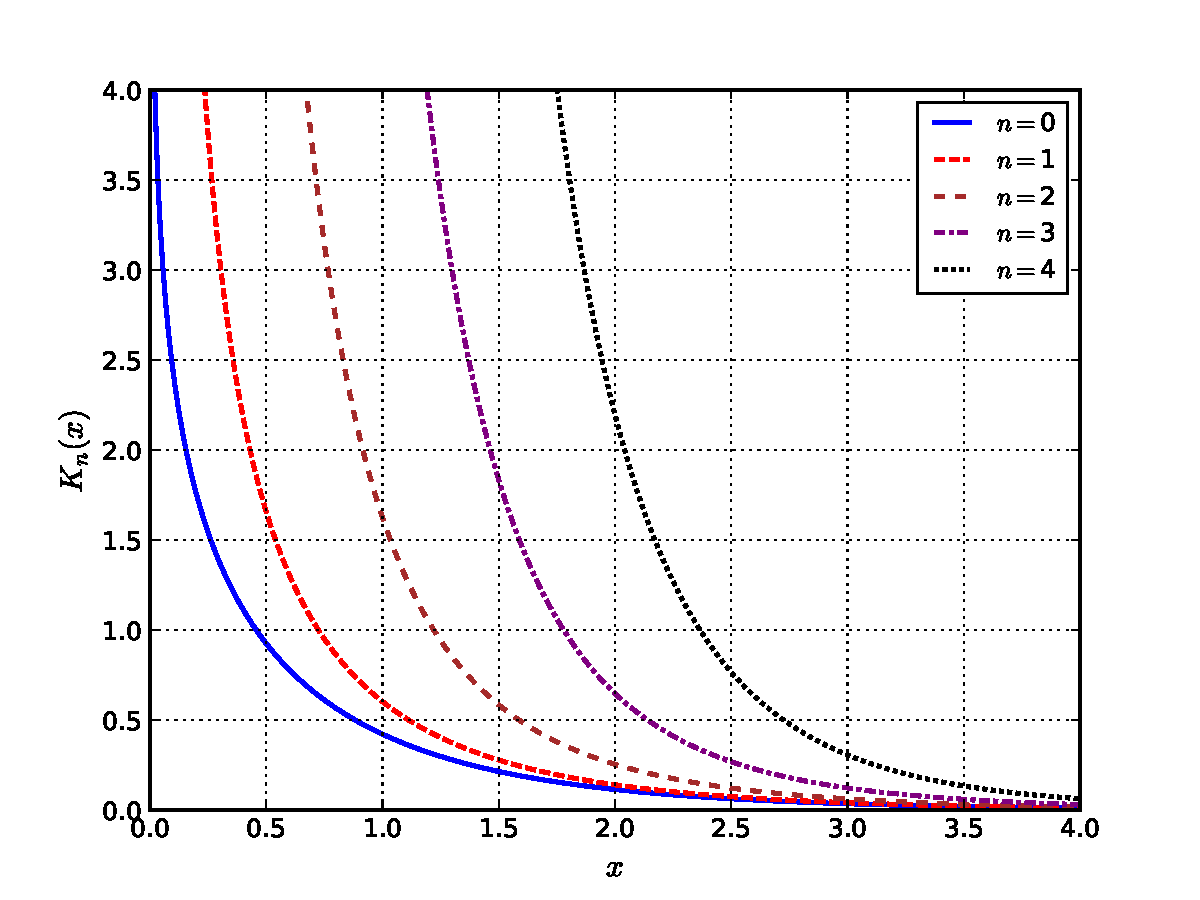
\includegraphics[angle=0,width=0.7\textwidth]{figs/fig-Bessel-K.pdf}
\caption{Primeras cinco funciones modificadas de Bessel de segunda primera especie y orden entero.}
\label{fig-Kn}
\end{figure}
Las funciones $K_\nu(x)$ satisfacen las siguientes relaciones de recurrencia
\begin{equation}\label{rrKnu1}
K_{\nu-1}(x)+K_{\nu+1}(x)=-2K'_\nu(x),
\end{equation}
\begin{equation}\label{rrKnu2}
K_{\nu-1}(x)-K_{\nu+1}(x)=-\frac{2\nu}{x}K_\nu(x),
\end{equation}
como puede verificarse a partir de \eqref{rrInu1}, \eqref{rrInu2}, \eqref{defKnu} y \eqref{Knder}. Note la diferencia de signo de estas relaciones con respecto a las correspondientes a las funciones de primera especie, \eqref{rrInu1} y \eqref{rrInu2}.

\section{Funciones Esf'ericas de Bessel}
Como vimos, en coordenadas esf'ericas la ecuaci'on radial proveniente de la separaci'on de variables de la ecuaci'on de Helmholtz es \eqref{ecrHelmce}. Adem'as, las soluciones finitas en $\theta=0$ y $\theta=\pi$ (es decir, sobre el eje $z$) de \eqref{ecThHelm} requieren que $Q=n(n+1)$. La ecuaci'on resultante tiene entonces soluciones de la forma
%\begin{equation}
%x^2 \frac{d^2 y}{dx^2} + 2x \frac{dy}{dx} + [x^2 - n(n+1)]y = 0.
%\end{equation}
\begin{equation}
R_n(r) = \frac{u_n(kr)}{\sqrt{r}} ,
\end{equation}
donde $k=\sqrt{|\alpha|}$ y $u_n(x)$ es soluci'on de la ecuaci'on (modificada, si $\alpha<0$) de Bessel de orden semientero, $\nu=n+1/2$.

En el caso en que $\alpha>0$, las soluciones $u(x)$ ser'an entonces combinaciones de funciones de Bessel de primera y segunda especie. Por esto, es conveniente definir las funciones esf'ericas de Bessel (de primera y segunda especie) por:
\begin{equation}
j_{n}(x) := \sqrt{\frac{\pi}{2x}} J_{n+1/2}(x),
\end{equation}
\begin{equation}
n_{n}(x) := \sqrt{\frac{\pi}{2x}} N_{n+1/2}(x) = (-1)^{n+1} \sqrt{\frac{\pi}{2x}} J_{-n-1/2}(x).
\end{equation}
El factor $\sqrt{\pi/2}$ es incluido por conveniencia, ya que entonces (ver \eqref{J1/2} y \eqref{J-1/2}) las primeras funciones resultan ser simples:
\begin{equation}\label{j0n0}
j_0(x) = \frac{\sen x}{x}, \qquad n_0(x)=-\,\frac{\cos x} {x}.
\end{equation}
Podemos encontrar una expresi'on en serie simple a partir\footnote{y usando la ``f'ormula de duplicaci'on de Legendre'', ver por ejemnplo ec. (10.66b) de \cite{Arfken}: $\Gamma(z+1)\Gamma(z+1/2)\equiv 2^{-2z}\pi^{1/2}\Gamma(2z+1)$, con $z=k+n+1/2$.} de \eqref{Besselnu},
\begin{align}
J_{n+1/2} (x)&= \sum_{k = 0}^\infty \frac{ (-1)^k }{ k! \Gamma(k + n + 3/2) }
\left( \frac{x}{2} \right)^{2k+n+1/2} \\
&=\sqrt{\frac{x}{2}} \sum_{k=0}^\infty \frac{ (-1)^k }{ k! \Gamma(k + n + 3/2) }
\left( \frac{x}{2} \right)^{2k+n} \\
&=\sqrt{\frac{x}{2}} \sum_{k=0}^\infty \frac{ (-1)^k }{ k!}\frac{2^{2k+2n+1}\Gamma(k+n+1)}{\pi^{1/2}\Gamma(2k+2n+2)}
\left( \frac{x}{2} \right)^{2k+n} \\
&=\sqrt{\frac{2x}{\pi}} 2^{2n}\sum_{k=0}^\infty \frac{(-1)^k }{k!}\frac{2^{2k}(k+n)!}{(2k+2n+1)!}\left(\frac{x}{2}\right)^{2k+n} \\
&=\sqrt{\frac{2x}{\pi}} 2^n x^n\sum_{k=0}^\infty \frac{(-1)^k}{k!}\frac{(k+n)!}{(2k+2n+1)!}x^{2k} .
\end{align}
Por lo tanto,
\begin{equation}
\boxed{j_n(x)=2^n x^n\sum_{k=0}^\infty \frac{(-1)^k}{k!}\frac{(k+n)!}{(2k+2n+1)!}x^{2k} .}
\end{equation}

An'alogamente, para la funci'on esf'erica de segunda especie, encontramos
\begin{equation}
\boxed{n_n(x)=\frac{(-1)^{n+1}}{2^nx^{n+1}}\sum_{k=0}^\infty \frac{(-1)^k(k-n)!}{k!(2k-2n)!}x^{2k} .}
\end{equation}

\subsection{Relaciones de Recurrencia}
A partir de las relaciones de recurrencia para $J_\nu$ y $N_\nu$, ver \eqref{rrJnu1}, \eqref{rrJnu2}, \eqref{rrNnu1} y \eqref{rrNnu2}, podemos derivar directamente las correspondientes relaciones para las funciones esf'ericas, obteniendo:
\begin{equation}
j_{n-1}(x)+j_{n+1}(x)=\frac{2n+1}{x}j_n(x), \qquad nj_{n-1}(x)-(n+1)j_{n+1}(x)=(2n+1)j'_n(x).
\end{equation}
Similarmente \eqref{Jnu-1JpJ2} y \eqref{rrJni+2} implican que
\begin{equation}
j_{n-1}(x)=x^{-n-1}\frac{d\ }{dx}\left[x^{n+1}j_n(x)\right],
\end{equation}
\begin{equation}\label{jn+1jn}
j_{n+1}(x)=-x^{n}\frac{d\ }{dx}\left[x^{-n}j_n(x)\right].
\end{equation}
Aplicando sucesivamente \eqref{jn+1jn} obtenemos una expresi'on en t'erminos de la funci'on $j_0(x)$:
\begin{equation}
j_n(x) = (-x)^n \left(\frac{1}{x}\frac{d}{dx}\right)^n\,j_0(x) .
\end{equation}
Similarmente,
\begin{equation}
n_n(x) = (-x)^n \left(\frac{1}{x}\frac{d}{dx}\right)^n\,n_0(x).
\end{equation}

\subsection{Expresiones expl'icitas}

De este modo, usando \eqref{j0n0} encontramos las siguientes 'utiles expresiones:
\begin{equation}
\boxed{j_n(x) = (-x)^n \left(\frac{1}{x}\frac{d}{dx}\right)^n\,\frac{\sen x}{x},}
\end{equation}
\begin{equation}
\boxed{n_n(x) = -(-x)^n \left(\frac{1}{x}\frac{d}{dx}\right)^n\,\frac{\cos x}{x}.}
\end{equation}
De este modo, podemos calcular expl'icitamente las funciones que necesitemos. Por ejemplo:
\begin{align}
j_0(x) &= \frac{\sen x}{x}, \\
j_1(x) &= \frac{\sen x} {x^2}- \frac{\cos x} {x}, \\
j_2(x) &= \left(\frac{3} {x^2} - 1 \right)\frac{\sen x}{x} - \frac{3\cos x} {x^2}, \\
j_3(x) &= \left(\frac{15}{x^3} - \frac{6}{x} \right)\frac{\sen x}{x} -\left(\frac{15}{x^2} - 1\right) \frac{\cos x} {x},
\end{align}
\begin{align}
n_0(x) &= -j_{-1}(x)=-\,\frac{\cos x} {x} ,\\
n_1(x) &= j_{-2}(x)=-\,\frac{\cos x} {x^2}- \frac{\sen x} {x}, \\
n_2(x) &=-j_{-3}(x)=\left(-\,\frac{3}{x^2}+1 \right)\frac{\cos x}{x}- \frac{3 \sen x} {x^2}, \\
n_{3}(x) &= j_{-4}(x) =\left( -\frac{15}{x^{3}}+\frac{6}{x}\right) \frac{\cos
x}{x}-\left( \frac{15}{x^{2}}-1\right) \frac{\sen x}{x}.
\end{align}
\begin{figure}[H]
\centering
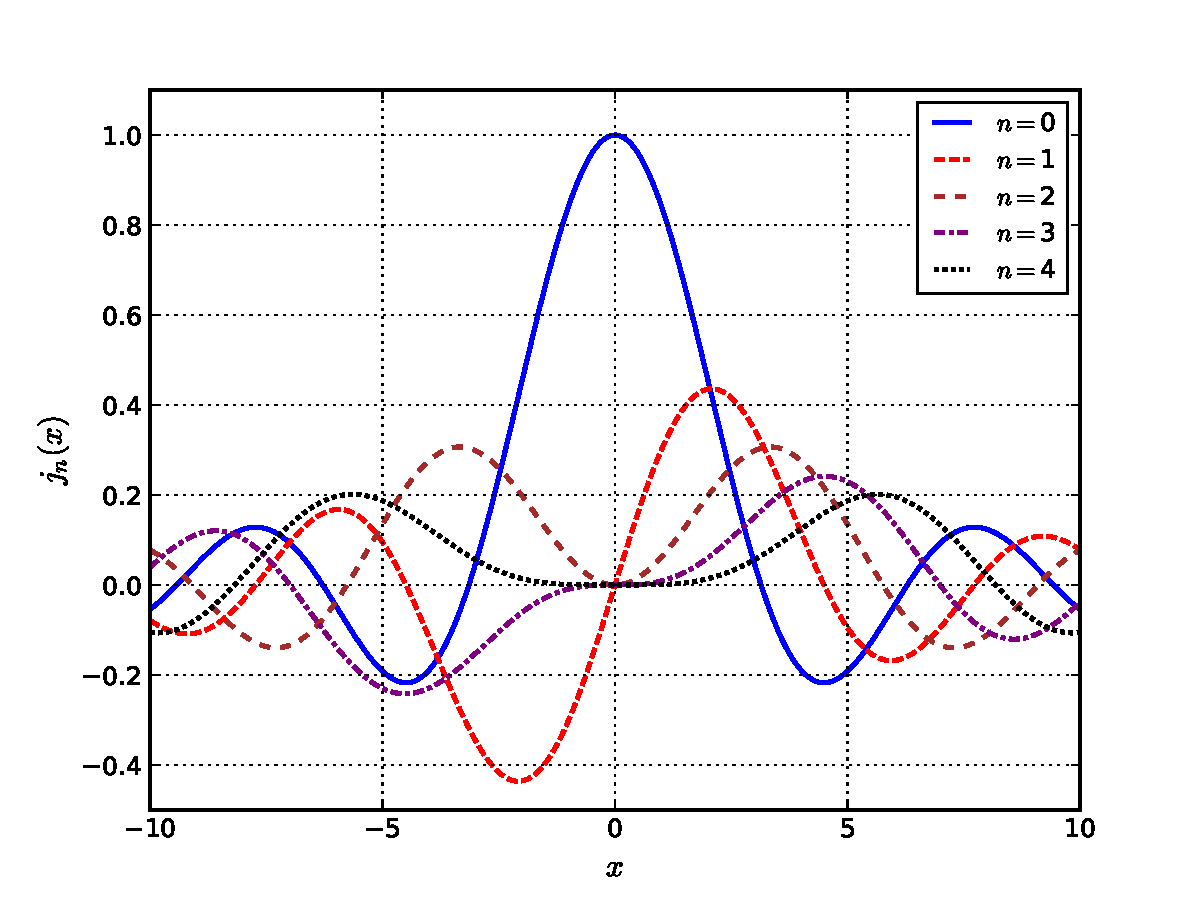
\includegraphics[angle=0,width=0.7\textwidth]{figs/fig-Bessel-Esferica-j.pdf}
\caption{Primeras cinco funciones esf'ericas de Bessel de primera especie de orden entero.}
\label{fig-jn}
\end{figure}
%
\begin{figure}[H]
\centering
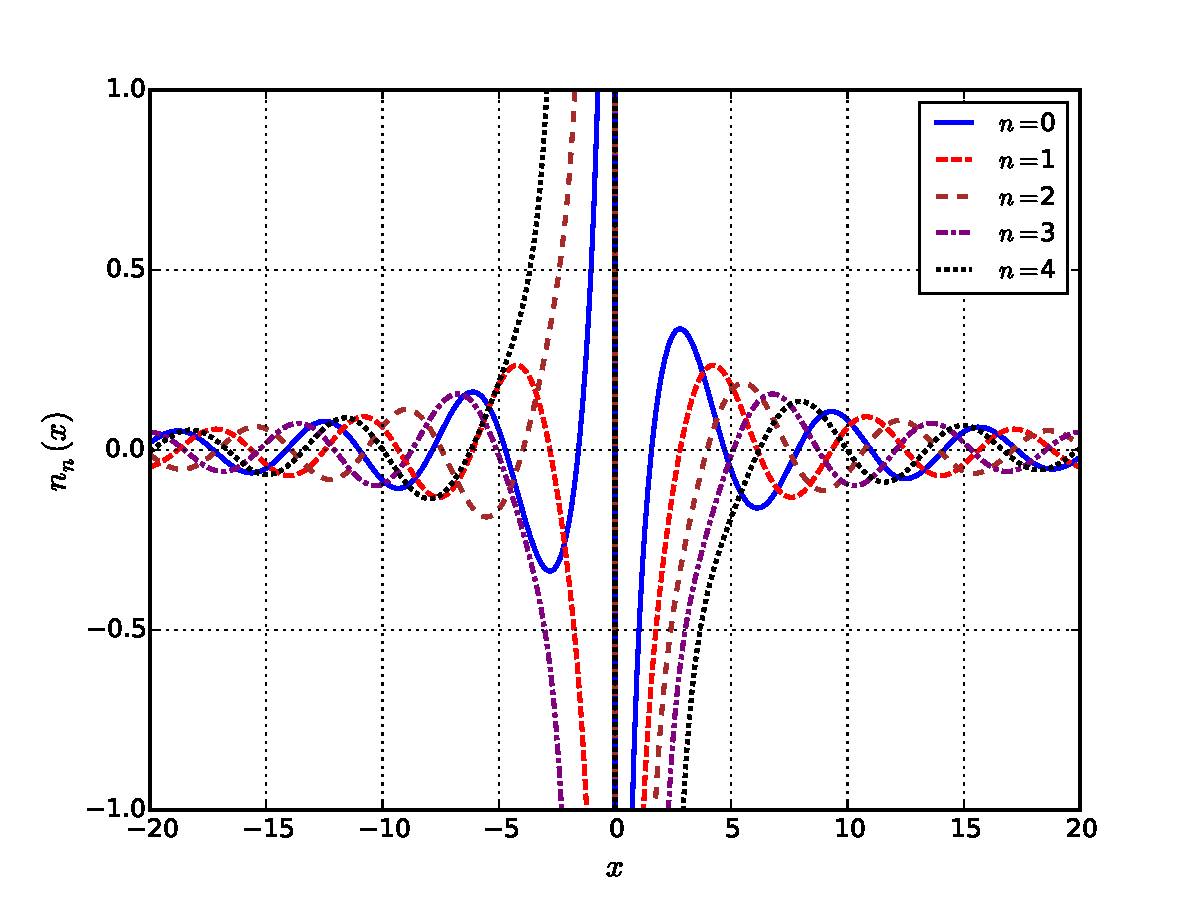
\includegraphics[angle=0,width=0.7\textwidth]{figs/fig-Bessel-Esferica-n.pdf}
\caption{Primeras cinco funciones esf'ericas de Bessel de segunda especie (funciones de Newmann) de orden entero.}
\label{fig-nn}
\end{figure}


\subsection{Relaciones de Ortogonalidad}
Nuevamente, podemos encontrar relaciones v'alidas para las funciones esf'ericas a partir de aquellas derivadas para las funciones de Bessel $J_\nu$. A partir de \eqref{roJnualpha} se sigue directamente que
\begin{equation}\label{rojnualpha}
\boxed{\int_0^a j_n\left(\frac{\bar{\alpha}_{n,m}}{a}r\right)j_n\left(\frac{\bar{\alpha}_{n,m'}}{a}r\right)r^2\,dr
=\delta_{m,m'}\frac{a^3}{2}\left[j_{n+1}(\bar{\alpha}_{n,m})\right]^2,}
\end{equation}
donde $\bar{\alpha}_{n,m}$ denota la $m$-'esima raiz de la la funci'on esf'erica $j_n(x)$. Ya que $j_n$ es proporcional a $J_{n+1/2}$, entonces $\bar{\alpha}_{n,m}=\alpha_{n+1/2,m}$.


\subsection{Funciones esf'ericas de Hankel} 
\begin{align}
h_n^{(1)}(x) &= j_n(x) + i n_n(x) , \\
h_n^{(2)}(x) &= j_n(x) - i n_n(x).
\end{align}
\begin{equation}
h_n^{(1)}(x) = (-i)^{n+1} \frac{e^{ix}}{x} \sum_{m=0}^n \frac{i^m}{m!(2x)^m} \frac{(n+m)!}{(n-m)!}
\end{equation}

\subsection{Forma asint'otica}
Para $x\ll 1$,
\begin{align}
j_n(x) &\approx \frac{2^nn!}{(2n+1)!}x^n, \\
n_n(x) &\approx -\frac{(2n)!}{2^nn!}\frac{1}{x^{n+1}}.
\end{align}
Para $x\gg n(n+1)$,
\begin{align}
j_n(x) &\approx \frac{1}{x}\sen\left(x-\frac{n\pi}{2}\right), \\
n_n(x) &\approx -\frac{1}{x}\cos\left(x-\frac{n\pi}{2}\right), \\
h^{(1)}_n(x) &\approx -\frac{i}{x}e^{i(x-{n\pi}/{2})}=(-i)^{n+1}\frac{e^{ix}}{x}, \\
h^{(2)}_n(x) &\approx \frac{i}{x}e^{-i(x-{n\pi}/{2})}=(i)^{n+1}\frac{e^{-ix}}{x}.
\end{align}

\subsection{Funciones modificadas esf'ericas de Bessel}
\begin{equation}
i_n(x):=i^{-n}j_n(ix)=\sqrt{\frac{\pi}{2x}}I_{n+1/2}(x), \qquad 
k_n(x):=-i^{n}h^{(1)}(ix)=\sqrt{\frac{\pi}{2x}}K_{n+1/2}(x).
\end{equation}

\subsubsection{Relaciones de Recurrencia}
\begin{align}
i_{n-1}(x)-i_{n+1}(x) &= \frac{2n+1}{x}i_n(x),  \\
ni_{n-1}(x)+(n+1)i_{n+1}(x) &= (2n+1)i'_n(x),
\end{align}
\begin{align}
k_{n-1}(x)-k_{n+1}(x) &= -\frac{2n+1}{x}k_n(x),\\
nk_{n-1}(x)+(n+1)k_{n+1}(x) &= -(2n+1)k'_n(x),
\end{align}
\begin{equation}
i_{n+1}(x)=x^n\frac{d\ }{dx}(x^{-n}i_n), \qquad k_{n+1}(x)=-x^n\frac{d\ }{dx}(x^{-n}k_n).
\end{equation}


\subsubsection{Formas asint'oticas}
\begin{equation}
i_n(x)\approx\frac{2^nn!}{(2n+1)!}x^n, \qquad k_n(x)\approx\frac{(2n)!}{2^nn!}x^{-n-1}, \qquad x\ll 1,
\end{equation}
\begin{equation}
i_n(x)\approx \frac{e^x}{2x}, \qquad k_n(x)\approx \frac{-e^x}{x}, \qquad x\gg \frac{n(n+1)}{2}.
\end{equation}


\subsubsection{Expresiones expl'icitas}
\begin{equation}
i_n(x)=x^n\left(\frac{1}{x}\frac{d\ }{dx}\right)^n\frac{\senh x}{x}, \qquad 
k_n(x)=(-1)^nx^n\left(\frac{1}{x}\frac{d\ }{dx}\right)^n\frac{e^{-x}}{x},
\end{equation}
\begin{align}
i_0(x) &= \frac{\senh (x)}{x}, \\
i_1(x) &= \frac{\senh (x)}{x}-\cosh (x), \\
i_2(x) &=\frac{\cosh (x)}{x}-\frac{\senh (x) }{{x}^{2}}, \\
i_3(x) &= \frac{\senh (x)}{x}+\frac{3\,\senh (x) }{{x}^{3}}-\frac{3\,\cosh (x) }{{x}^{2}}, \\
i_4(x) &= -\frac{6\,\senh (x) }{{x}^{2}}-\frac{15\,\senh (x) }{{x}^{4}}+\frac{\cosh (x) }{x}+\frac{15\,\cosh (x) }{{x}^{3}},
\end{align}
\begin{align}
k_0(x) &= \frac{{e}^{-x}}{x} , \\
k_1(x) &= \frac{{e}^{-x}}{x}+\frac{{e}^{-x}}{{x}^{2}}, \\
k_2(x) &= \frac{{e}^{-x}}{x}+\frac{3\,{e}^{-x}}{{x}^{2}}+\frac{3\,{e}^{-x}}{{x}^{3}}, \\
k_3(x) &= \frac{{e}^{-x}}{x}+\frac{6\,{e}^{-x}}{{x}^{2}}+\frac{15\,{e}^{-x}}{{x}^{3}}+\frac{15\,{e}^{-x}}{{x}^{4}}, \\
k_4(x) &= \frac{{e}^{-x}}{x}+\frac{10\,{e}^{-x}}{{x}^{2}}+\frac{45\,{e}^{-x}}{{x}^{3}}+\frac{105\,{e}^{-x}}{{x}^{4}}+\frac{105\,{e}^{-x}}{{x}^{5}}.
\end{align}
\begin{figure}[H]
\centering
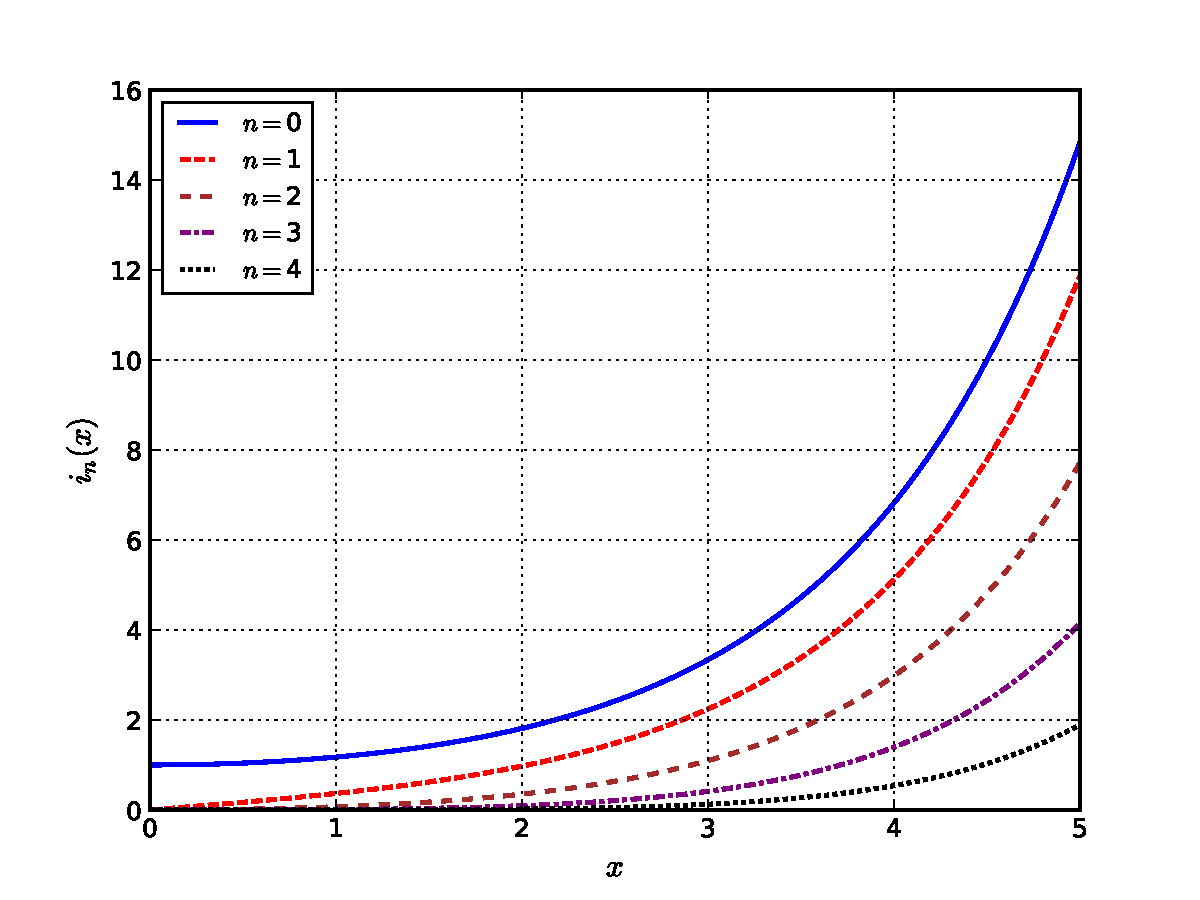
\includegraphics[angle=0,width=0.7\textwidth]{figs/fig-Bessel-Esferica-i.pdf}
\caption{Primeras cinco funciones esf'ericas modificadas de Bessel de primera especie de orden entero.}
\label{fig-in}
\end{figure}
%
\begin{figure}[H]
\centering
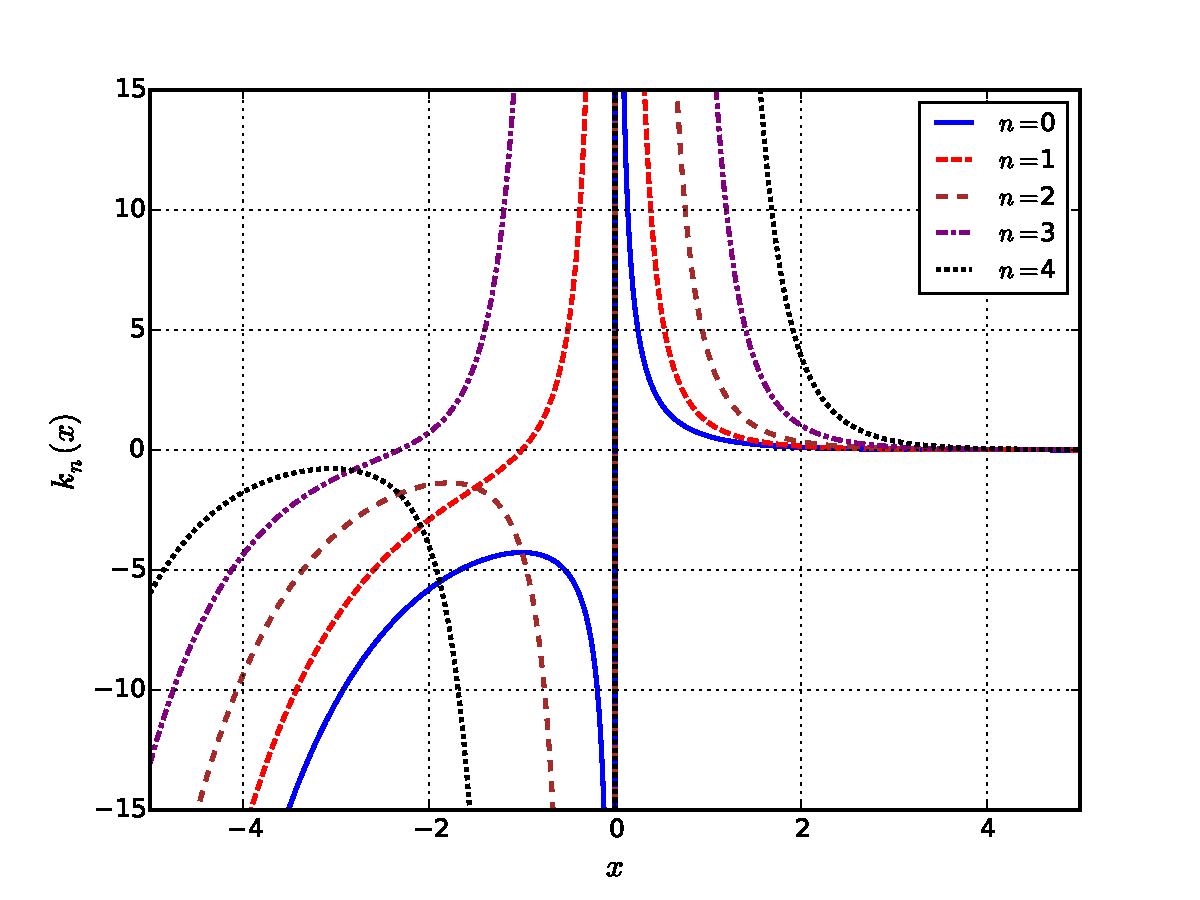
\includegraphics[angle=0,width=0.7\textwidth]{figs/fig-Bessel-Esferica-k.pdf}
\caption{Primeras cinco funciones esf'ericas modificadas de Bessel de segunda especie (funciones de Newmann) de orden entero.}
\label{fig-kn}
\end{figure}